%%!TEX encoding = UTF-8 Unicode

\documentclass[a4paper,11pt]{article}
\input{../../preambule.tex}
\input{../../figures.tex}



\lhead{\ccby}
\rhead{\small{ $1^{\text{ère}}$ NSI}}
\chead{\small{ $C05$ Tuples, tableaux et algorithmes de tableaux}}


\lfoot{\tiny{Ann\'ee 2020-2021}}
\cfoot{\textbf{Page \thepage/\pageref{LastPage}}}
%\cfoot{}
\rfoot{\tiny{www.zonensi.fr}}

\begin{document}
\sffamily %Pourutiliser une police sans empatement
\begin{center}
 \large{\textbf{$C05-04$ Tableaux à deux dimensions}}
\end{center}


\begin{definition}{Matrices}
\parbox{0.65\linewidth}{
 \noindent En mathématiques, on appelle \textbf{matrice} un tableau $M$ de nombres $a_{i,j}$ où $i$ est le numéro de ligne et $j$ le numéro de colonne. On parlera de matrice de dimension $m\times n$ si la matrice possède $m$ lignes et $n$ colonnes.\\
 }\hfill\parbox{0.3\linewidth}{
 \begin{center}
 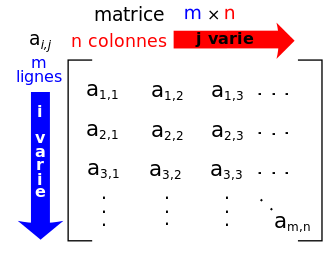
\includegraphics[width=0.9\linewidth]{Matrice.png}
 \end{center}
 }
\end{definition}
\begin{info}{Représentation informatique}
 Pour représenter informatiquement une matrice de nombres, entiers ou flottant, on utilise un tableau de tableau. Ainsi la matrice $M = \begin{pmatrix}
1&2&3\\
4&5&6                                                                                                                                        \end{pmatrix}$ sera représentée sous la forme suivante :
 \begin{center}
  \texttt{ M = [[1, 2, 3], [4, 5, 6]]}
 \end{center}
En Python, il est souvent préférable de définir une matrice en utilisant la possibilité de sauter des lignes à l'intérieur de deux délimiteurs :
\begin{lstlisting}[language=python, caption = {Matrice}]
>>> M = [[1, 2, 3],
	[4, 5, 6]]		
\end{lstlisting}

On peut alors accéder aux éléments de la matrice par la notation suivante :
\begin{lstlisting}[language=python, caption = {Eléments}]
>>> M[1][2]
6
\end{lstlisting}
Ici \texttt{M[1][2]} indique d'aller chercher l'élément  d'indice 2 de la liste d'indice 1 de M, où autrement dit l'élément de \textbf{la ligne d'indice 1 et de colonne d'indice 2}.
\end{info}
\begin{ExerciceNomme}{Lire une matrice}
On considère la matrice suivante :
\begin{lstlisting}[language=python, caption = {Exercice}]
>>> M =[[1, 2, 3, 4, 5],
 	[2, 4, 6, 8, 10],
 	[3, 6, 9, 12, 15],
	[4, 8, 12, 16, 20]]
\end{lstlisting}
\begin{enumerate}
\item A quel nombre fait référence l'élément $M[1][3]$ ? \caserepsanssaut{2}{0.5}
\item Comment obtenir le nombre $15$  ? \caserepsanssaut{2}{0.5}
\item A quel nombre fait référence l'élément $M[-1][2]$ ? \caserepsanssaut{2}{0.5}
\item A quel nombre fait référence l'élément $M[0][-2]$ ? \caserepsanssaut{2}{0.5}
\end{enumerate}
\end{ExerciceNomme}
\begin{ExerciceNomme}{Parcourir une matrice}
Pour parcourir une matrice, il faut utiliser deux boucles \texttt{for} imbriquées l'une dans l'autre :
\begin{enumerate}
\item Tester le code suivant sur une matrice $M = \begin{pmatrix}
1&2&3\\
4&5&6                                                                                                                                        \end{pmatrix}$ 
\begin{lstlisting}[language=python, caption = {parcours ligne}]
>>> for i in range(2) :
	for j in range(3) :
		print(M[i][j])
\end{lstlisting}
Dans quel ordre apparaissent les éléments ? \caserepsanssaut{4}{0.5}


\item Tester le code suivant, toujours sur la matrice $M$
\begin{lstlisting}[language=python, caption = {parcours colonnes}]
>>> for j in range(3) :
	for i in range(2) :
		print(M[i][j])
\end{lstlisting}
Dans quel ordre apparaissent les éléments ? \caserepsanssaut{4}{0.5}
\item Dans le code précédent, que se passe-t-il si on écrit \texttt{print(M[j][i])} ? \caserepsanssaut{4}{0.5}
\item Tester le code suivant, toujours sur la matrice $M$
\begin{lstlisting}[language=python, caption = {foreach}]
>>> for line in M :
	for elem in line :
		print(elem)
\end{lstlisting}
Dans quel ordre apparaissent les éléments ? \caserepsanssaut{4}{0.5}
\item Est-il possible d'inverser le type de parcours ?\caserepsanssaut{2}{0.5}
\item Tester le code suivant, toujours sur la matrice $M$
\begin{lstlisting}[language=python, caption = {foreach et enumerate}]
>>> for i, line in enumerate(M) :
	for j, elem in enumerate(line) :
		print(f"M[{i}][{j}] = {elem}")
\end{lstlisting}
A quoi sert la fonction \texttt{enumerate} ?
\caserep{\linewidth}{1.5}
\end{enumerate}
\end{ExerciceNomme}
\begin{ExerciceNomme}{Initialisation de matrices}


\begin{info}{Pourquoi initialiser}
très souvent on va travailler sur un tableau et/ou une matrice dont on connait au préalable la dimension, et sur laquelle on va modifier les valeurs au fur et à mesure. Il sera souvent plus facile de travailler sur une matrice déjà pré-remplie avec des valeurs de départ - des zéros souvent, plutôt que d'être obligé de vérifier que le terme $a(i][j]$ existe, et de faire un \texttt{append} dans le cas contraire.
\end{info}
\begin{enumerate}
\item Avec des tableaux à une dimension :
\begin{enumerate}
\item Tester la ligne suivante :
\begin{lstlisting}[language=python, caption = {Initialisation de tableau}]
>>> T = [0]*10
\end{lstlisting}
Que fait ce code ?
\caserep{\linewidth}{1}
\item Compléter le code afin d'affecter à chaque nombre du tableau le cube de son indice :
\caserep{\linewidth}{3}
\end{enumerate}
\item Avec des tableaux à deux dimensions :
\begin{enumerate}
\item Tester la ligne suivante :
\begin{lstlisting}[language=python, caption = {En dimension 2}]
>>> M = [[0]*10]*4
\end{lstlisting}
Que fait ce code ?
\caserep{\linewidth}{1}
\item Tester alors la ligne suivante :
\begin{lstlisting}[language=python, caption = {Affectations 1}]
>>> M[0][5] = 777
\end{lstlisting}
\item A quoi est-alors associé le nom $M$ ? \caserep{\linewidth}{1}
\item Quel est le problème ?\caserep{\linewidth}{2}
\item Tester alors le code suivant, :
\begin{lstlisting}[language=python, caption = {Une bonne initialisation}]
>>> M = [[0]*10 for i in range(4)]
\end{lstlisting}
\item Faites de nouveau l'affectation suivante
\begin{lstlisting}[language=python, caption = {Affectations 1}]
>>> M[0][5] = 777
\end{lstlisting}
le résultat est-il conforme aux attentes ? \caserepsanssaut{4}{0.5}
\end{enumerate}
\end{enumerate}
\end{ExerciceNomme}
\begin{ExerciceNomme}{Carré magiques}
Un carré magique d'ordre $n$ est une matrice carrée $n\times n$ telle que que la somme des nombres sur chaque ligne, sur chaque colonne et sur chaque diagonale principale soient égales.
\begin{enumerate}
\item Vérifier que la matrice $\begin{pmatrix} 4&9&2\\3&5&7\\8&1&6\end{pmatrix}$ est bien un carré magique.
\item On se propose de construire une fonction vérifiant qu'une matrice de taille $n \times n$ est bien un carré magique.
\begin{enumerate}
\item Créer une fonction \texttt{estCarre(M)} qui vérifie que la matrice $M$ est bien carrée (son nombre de ligne est égal à son nombre de colonne). Cette fonction renverra \texttt{True} dans ce cas, et \texttt{False} sinon.
\item Créer une fonction \texttt{sommeLigne(M,i)} qui renvoie la somme des nombres de la ligne $i$ de la matrice $M$.
\item Créer une fonction \texttt{sommeColonne(M,i)} qui renvoie la somme des nombres de la colonne $i$ de la matrice $M$.
\item Créer une fonction \texttt{sommeDiagPrincipale(M)} qui renvoie la somme des nombres de la \textit{diagonale principale} de $M$ (diagonale dont les éléments ont le même numéro de ligne et de colonne).
\item Créer une fonction \texttt{sommeDiagSecondaire(M)} qui renvoie la somme des nombres de la diagonale non principale de $M$.
\item En utilisant les fonctions précédentes, créer une fonction \texttt{estMagique(M)} qui renvoie \texttt{True} si la matrice $M$ est magique, et \texttt{False} sinon.
\end{enumerate}
\end{enumerate}
\begin{info}{D'autres carrés magiques}
Vous trouverez des carrés magiques de différents ordres sur les pages suivantes :
\trianglenoir
\begin{itemize}
\item la page wikipédia des carrés magiques ( mathématiques) \includegraphics[scale=0.2]{wikipedia_CM.png}
\item \url{http://www.bibmath.net/carres/}
\item \url{http://www.maths-rometus.org/mathematiques/maths-et-jeux/carres-magiques.asp#id1781}
\end{itemize}
\end{info}
\end{ExerciceNomme}
\end{document}
